%%% TeX-master: "../main.tex"
% kapitel5.tex
\chapter{Konkret getestete Applikationen}\label{chapter:concretetests}


Dieses Kapitel


\section{Resultate}\label{section:testresults}

\begin{figure}
	\centering
	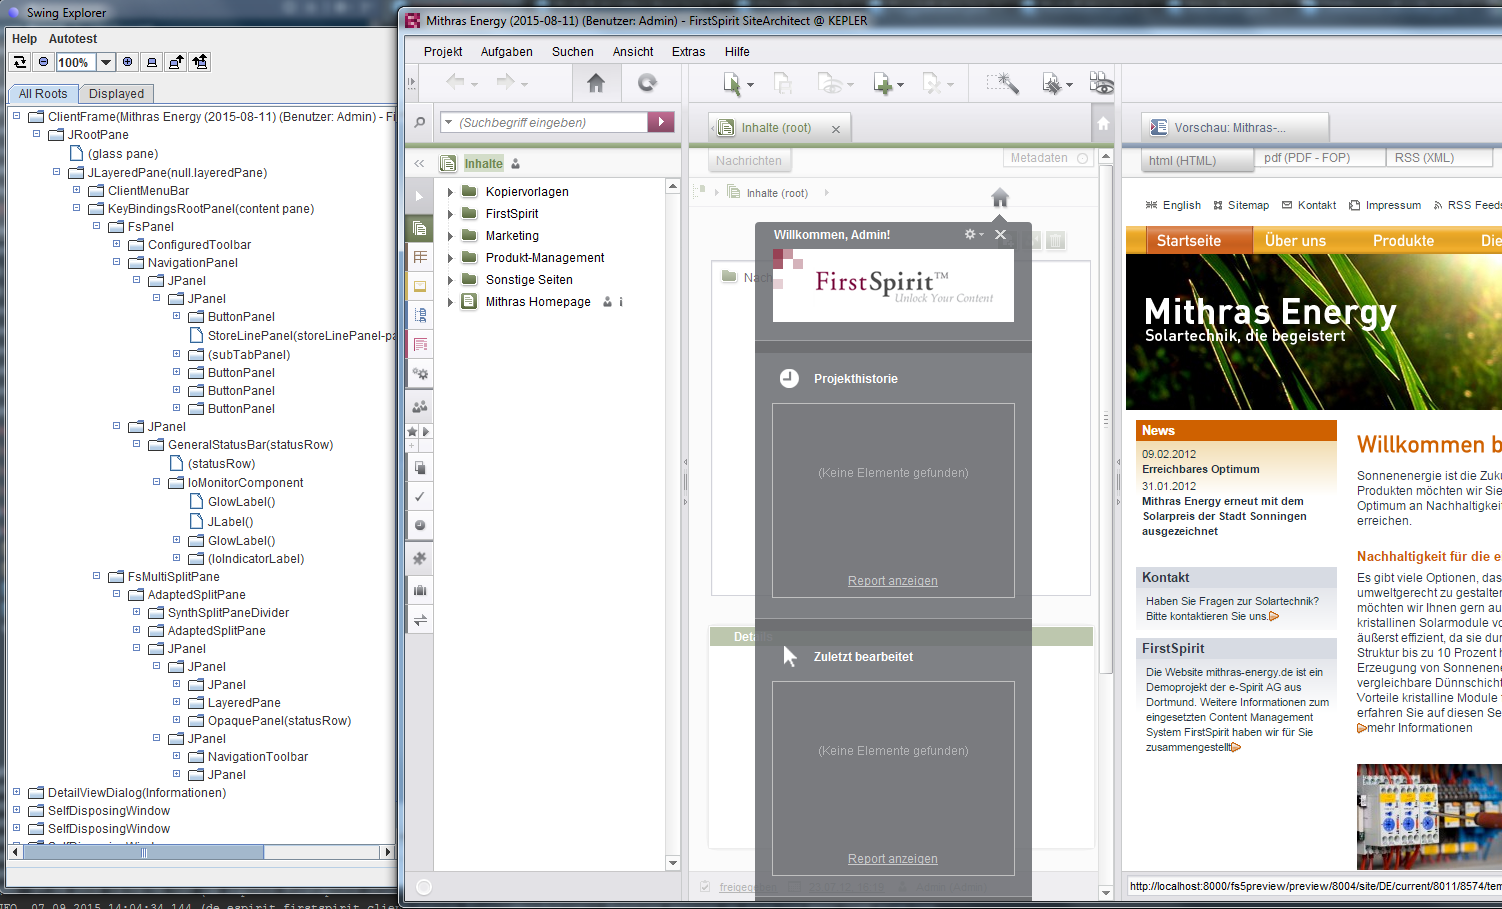
\includegraphics[width=0.85\textwidth]{bilder/screenshot_freespirit.png}
	\caption{Screenshot der e-Spirit CMS-Anwendung FirstSpirit \cite{website:firstspirit} 
	sowie anhängigem Swing Explorer, der den Komponentenbaum der Applikation darstellt}
	\label{fig:screenshot_freespirit}
\end{figure}

\begin{figure}
	\centering
	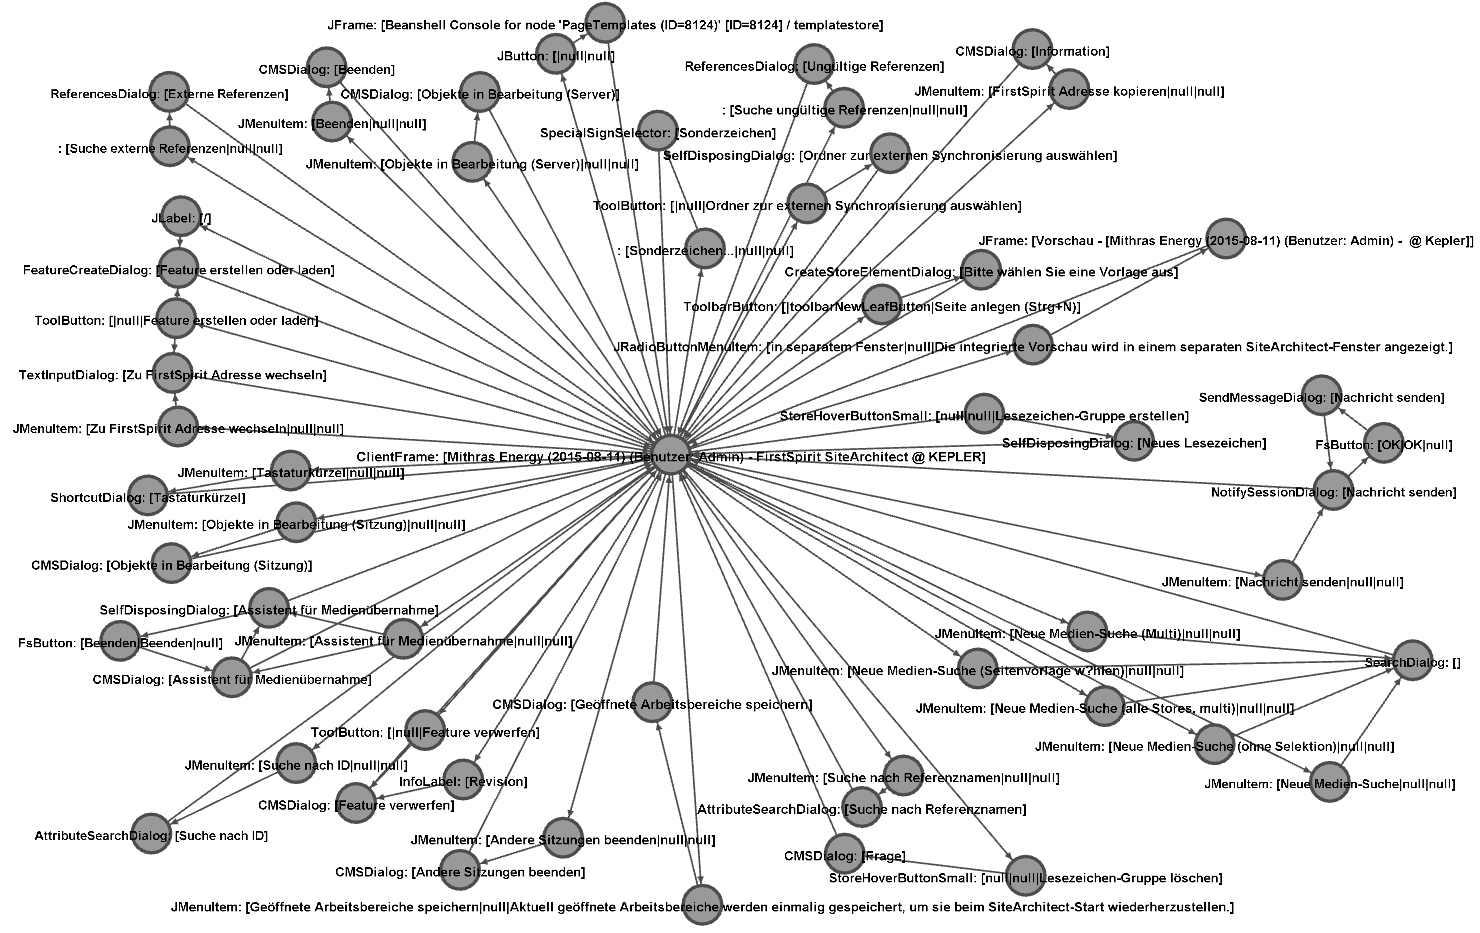
\includegraphics[width=0.85\textwidth]{bilder/model_freespirit.png}
	\caption{mit Gephi \cite{website:gephi} und dem Yifan Hu Algorithmus \cite{hu2005efficient}
    sowie noch für Lesbarkeit maneull angepasste visualierte Graphausgabe 
	des Autotesters über FirstSpirit bei einem der ergiebigeren Durchläufe.}
	\label{fig:model_freespirit_06.10.2015}
\end{figure}



Die Knoten sind in Dreiergruppen angeordnet: Ein Ursprungsfenster, ein Übergangsknoten
(bzw. ein Wort des Modells), sowie der resultierende Zustand bzw. das sich öffnende Fenster.
Dies ist schlicht eine Frage der Lesbarkeit - anstelle der mittleren Knoten für Übergänge sollten
eigentlich schlicht beschriftete Kanten benutzt werden, aber dies schränkt die Möglichkeiten,
den anhängigen Text in eine lesbare Form zu bringen, zu stark ein.


\section{Vergleich mit klassischen Tests}\label{section:testcomparisonclassic}

